\documentclass[uplatex, a4paper, 12pt, openany, oneside]{jsbook}

\usepackage[dvipdfmx]{graphicx}
\usepackage[dvipdfmx]{color}
\usepackage[dvipdfmx, bookmarks=true, setpagesize=false, hidelinks]{hyperref}
\usepackage{pxjahyper}
\usepackage{amsmath}
\usepackage{amsthm}
\usepackage{amssymb}
\usepackage{cases}
\usepackage{thesis}
\usepackage{here}
\usepackage{url}


\thesis{インテリジェントロボットモーション}
\thema{レポート}
\title{
  \centering
    \scalebox{1.0}{軌道計画と軌道生成}\\
    \vspace{-0.3zh}
    \scalebox{0.6}{Path planning and Trajectory Generation}
    \vspace{-0.6zh}
}
\setlength{\textwidth}{\fullwidth}
\setlength{\evensidemargin}{\oddsidemargin}

\date{\today}
\vspace{-15.0zh}
\organization{千葉工業大学 先進工学部 未来ロボティクス学科}
\author{20C1117 望月悠矢}
\vspace{-15zh}

\renewcommand{\baselinestretch}{1.2}
\begin{document}

%% Front Matter
\frontmatter{}
%
\maketitle
%
%!TEX root = ../thesis.tex
\chapter*{概要}
\thispagestyle{empty}
%
\begin{center}
  \scalebox{1.5}{}\\
\end{center}
\vspace{1.0zh}
%

本レポートでは,インテリジェントロボットモーション第11回「軌道計画と軌道生成」の解説を行う.
マニピュレータロボットや移動型ロボットなどをある地点から目標地点まで動かすときにニュートン・オイラー法やラグランジュ法
を用いて導出した運動学に基づいてマニピュレータが出すトルクや力を計算するが,このように
計算された力は各時刻の力を表すものであり,ロボットは軌道を描くことはできず,ロボットの通るべき経路は考慮されない.したがって,ロボットの
通るべき「軌道」を「計画」し,その軌道上をロボットが追従するように出すべき力を連続な力で表し,「軌道」を「生成」する必要がある.
はじめに軌道計画(経路計画)と軌道計画の違いと概念について解説し,次に軌道計画の主要なアルゴリズムの基礎的な理論について簡単に紹介する.最後にbang-bang制御による軌道生成の解説を行う.

キーワード: ロボット,経路計画,軌道生成

%
\tableofcontents
%
\listoffigures
%

%
%% Main Matter
\mainmatter{}
%
\chapter{経路計画と軌道生成}
\label{chap:section1}
%
%\input{introduction/preface}
%
%!TEX root = ../thesis.tex

\section{第1章の導入}

運動学を導出し適用するだけでは,ロボットを適切に動作させることができない.
制御をするには人間が意図したとおりに動いてほしい.そのために用いられる方法が軌道計画(経路計画)と軌道生成である.
運動学だけでは適切に動作させることができないというのは,運動学はロボットが出す各時刻の力しか計算できないからである.
今回扱う軌道生成では各時刻の力ではなく,連続した時間の力を計算することができる.これによりロボットに連続的な動作をさせることができる.
その上で,ロボットが障害物などを回避し,ある地点から目的の地点までの軌道を決定するのが軌道計画(経路計画)である.

軌道計画(経路計画)と軌道生成には大きな違いがある.その違いについて,使用される英単語の違いから見ていく.
その後に経路計画と軌道生成についての解説を行う.
\newpage

\begin{figure}[hbtp]
  \centering
 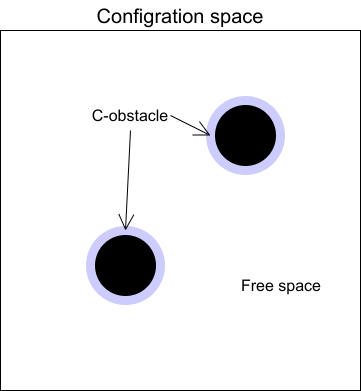
\includegraphics[keepaspectratio, scale=0.8]
      {images/png/ConfigrationSpace.drawio.png}
 \caption{Configration space}
 \label{Fig:ConfigrationSpace}
\end{figure}

経路計画では基本的にコンフィグレーション空間を使用する.
コンフィグレーション空間内にある障害物をC-obstacleと呼ぶ.
C-obstacleは実際の空間の障害物に対応しており,
障害物のギリギリに経路が計画されるのを防ぐため,
Fig.\ref{Fig:ConfigrationSpace}の水色の円のように実際の大きさよりも膨張させて用いられることが多い.

\newpage

%!TEX root = ../thesis.tex

\subsection{経路と軌道の違い}

軌道に対応する英単語として"Path"と"Trajectory"という単語が挙げられる.
この2つの英単語は運動の計画において違う意味を持ち,その意味は以下のようになる.
\begin{quote}
     \begin{itemize}
      \item Path:ロボットがどこを通るか
      \item Trajectory:ロボットがどのような運動で通るか
     \end{itemize}
\end{quote}
このように,"Path"と"Trajectory"には違いがあり,これらを日本語で再定義すると,"Path"は「経路」,
"Trajectory"は「軌道」とすることができる.そして,ロボットがどこを通るかを計画することを"Path planning",ロボットがどのような運動で通るかを決めることを"Trajectory generation"
と呼ぶ.以降,区別を明確にするために"Path planning"を「経路計画」,"Trajectory generation"を「軌道生成」と呼ぶことにする.
\newpage

%!TEX root = ../thesis.tex

\subsection{経路計画とは}

\begin{figure}[hbtp]
  \centering
 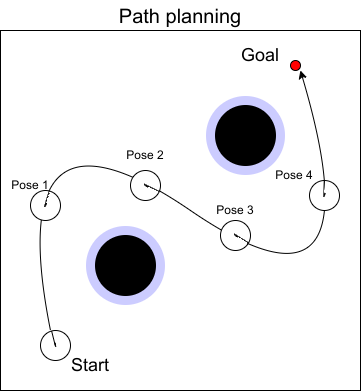
\includegraphics[keepaspectratio, scale=0.8]
      {images/png/PathPlanning.drawio.png}
 \caption{Path planning}
 \label{Fig:PathPlanning}
\end{figure}

経路計画は前述したように,ロボットがどのように通るかを計画することである.経路計画では,
ロボットの姿勢と位置,スタートからゴールまでにある障害物が考慮されたスタート地点からゴールまでの最短な経路が計画される.
計画された経路はロボットが通るべき位置,そのときに取るべき姿勢とその地点を通る順番の3つの条件からなる
複数の点の集合であると言うことができる.

Fig.\ref{Fig:PathPlanning}は経路計画のイメージ図である.黒と青の円で表されているのが障害物であり,
円と線分で表されているのがロボットである.線分の向きがロボットの姿勢を表している.
Fig.\ref{Fig:PathPlanning}のように経路計画では,ロボットの姿勢と位置が順番に指定される.
\newpage

%!TEX root = ../thesis.tex

\subsection{軌道生成とは}

\begin{figure}[hbtp]
  \centering
 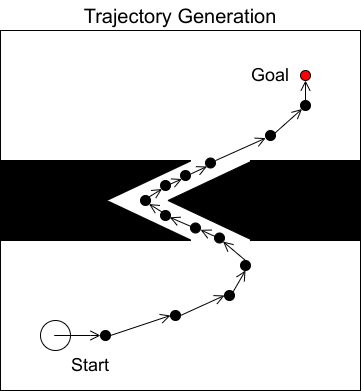
\includegraphics[keepaspectratio, scale=0.8]
      {images/png/TrajectoryGeneration.drawio.png}
 \caption{Trajectory Generation}
 \label{Fig:TrajectoryGeneration}
\end{figure}

軌道生成は,「1.1.1 経路と軌道の違い」で述べたように,ロボットがどのような運動で通るかを決めることである.
多くの経路計画ではロボットの運動学やメカニズムを無視しているため,ロボットの機構や特性で動作が難しい経路が計画されることがある.その例を以下に示す.
\begin{quote}
     \begin{itemize}
      \item アッカーマンリンクの自動車がその場で90°回転するような経路
      \item 対向二輪のロボットが姿勢を変えずに車輪に対して垂直に移動するような経路
      \item 等速で狭い場所も広い場所を通るような経路
     \end{itemize}
\end{quote}
そこで,ロボットが実際に動作及び制御可能な範囲で経路を追従させるために運動学やメカニズムを考慮した「軌道生成」を用いてロボットの運動
を決める.軌道生成を行うことで狭い道で速度を遅くしたり,広い道では速度を速くするといった動作や計画された経路の通過地点に対してロボットの機構や特性を
考慮した軌道を生成することができる.

Fig.\ref{Fig:TrajectoryGeneration}は軌道生成のイメージである.
黒い点がロボットの位置であり,矢印がロボットの速度,中央にある黒い部分が障害物である.
軌道生成ではこのようなロボットの軌道を生成することができる.
\newpage
%!TEX root = ../thesis.tex

\section{第1章のまとめ}

第一章では,"Path"と"Trajectory"の違い,経路計画と軌道生成について解説した.
"Path"はロボットどのように通るか,"Trajectory"はロボットがどのように運動するかという意味であった.
経路計画は障害物と位置と姿勢を考慮したロボットが通る経路を計画するものであった.
また,軌道生成はロボットの運動学,機構や特性を考慮した軌道を生成することであった.
\newpage

%

%ここにディレクトリのパスを追加していく
\chapter{経路計画のアルゴリズム}
\label{chap:section2}
%
%\input{introduction/preface}
%
%!TEX root = ../thesis.tex

\section{第2章の導入}

経路計画には様々なアルゴリズムがあり,ベースとなる理論も様々である.
それらの中で代表的なアルゴリズムの基礎理論である,ダイクストラ法やA*法に使用されるグラフ探索,
人工ポテンシャルを使用するポテンシャル法,RRTなどに使用されるランダムに配置した点を元に経路を決めるRRM,
以上の3種類のアルゴリズムの基礎的な理論について簡単に紹介する.

\newpage

%!TEX root = ../thesis.tex

\subsection{グラフ探索}

\begin{figure}[hbtp]
  \centering
 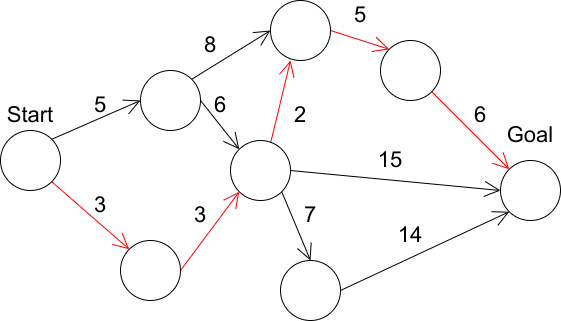
\includegraphics[keepaspectratio, scale=0.6]
      {images/png/Dijkstra.drawio.png}
 \caption{Connected graph}
 \label{Fig:Dijkstra}
\end{figure}

グラフ探索では,経由する点と点を結び最短な経路を探索する.
ここで点を「頂点」,点と点を結んで線にしたものを「パス」という.
グラフ探索ベースの経路計画では,
スタートの距離,すなわち重みを0として頂点間のパスに指定された重みに応じて頂点の重みが加算されていく.
最終的にゴールまでの重みが小さい経路が選択されそれが最短の経路であるという理論である.
Fig.\ref{Fig:Dijkstra}がそのイメージ図である.円が頂点,矢印がパスである.
現実的には,点がロボットが経由する地点で,矢印がロボットが移動する経路で重みがロボットが移動する距離である.
赤い矢印の経路が最も重みが小さいため,最短経路ということになる.

しかし,このアルゴリズムにはパスがロボットの運動として適切かどうかという問題がある.
すなわち,前述したロボットの機構や特性を無視したパスが生成される問題である.
それらの問題があってもスタートからゴールまでを最短距離で移動するには有用なアルゴリズムであり,ダイクストラ法やA*法で使用されている.
これらのアルゴリズムは大域経路計画としても使用されている.

グラフ探索の別の応用先としてはカーナビゲーションが挙げられる.
\newpage

%!TEX root = ../thesis.tex

\subsection{ポテンシャル法}

\begin{figure}[H]
  \centering
 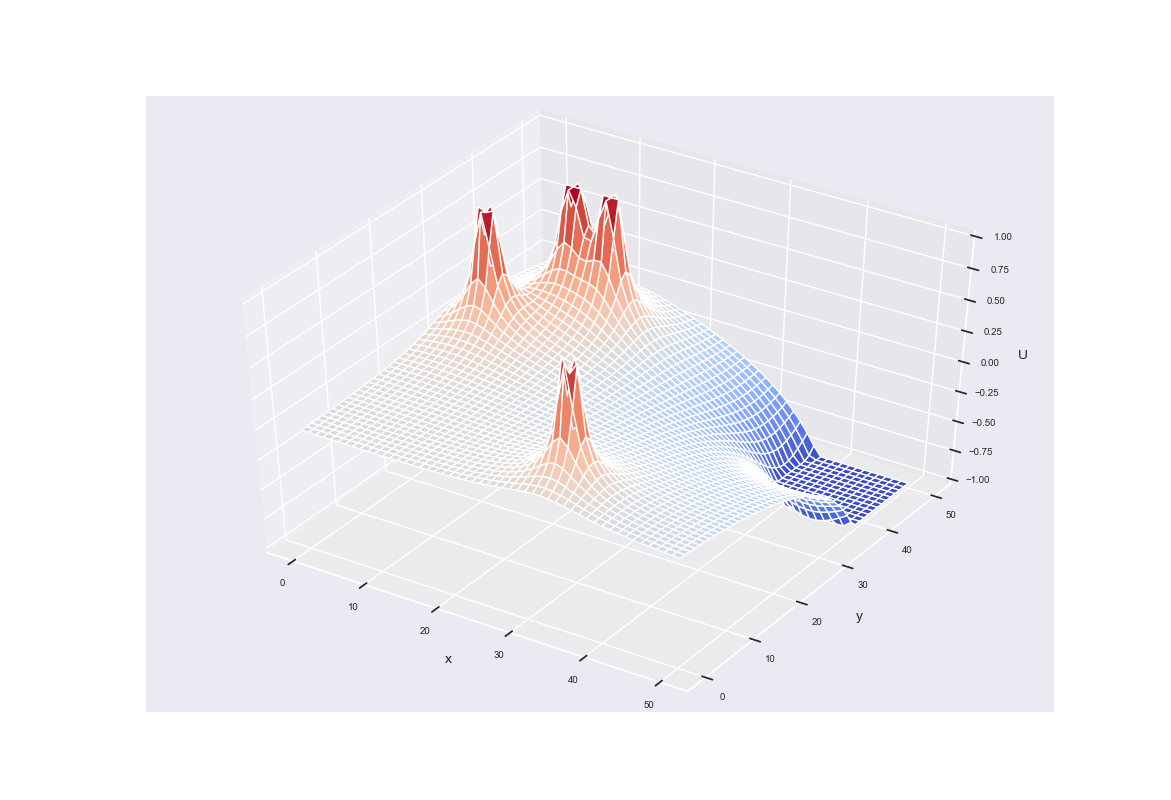
\includegraphics[keepaspectratio, scale=0.4]
      {images/png/potential.png}
 \caption{Potential field ~\cite{pathpt1:online}}
 \label{Fig:potential}
\end{figure}

ポテンシャル法は人工的に作り出したポテンシャル場を使用して,
スタートからゴールまでボールが転がる方向にロボットを移動させる方法である.
ポテンシャル場はゴールが谷底の斜面になっており,障害物は山になる.
スタートからボールを転がすと山と山の間の谷をコロコロと
谷底のゴールに向かって転がっていくというのがポテンシャル法のイメージである.

問題点としては,局所解であるローカルミニマムに陥ってしまうことが挙げられる.
これはゴールではない部分に谷底がもう一つできてしまう現象である.
このローカルミニマムを回避する方法は右手法など様々に研究されている.


\newpage

%!TEX root = ../thesis.tex

\subsection{RRM(Random Road Map)}

\begin{figure}[hbtp]
  \centering
 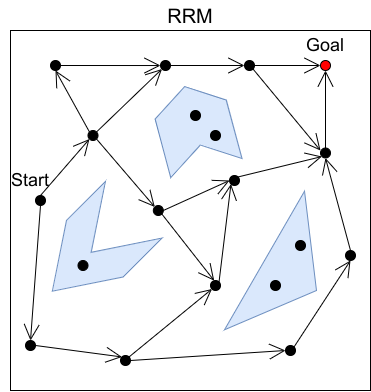
\includegraphics[keepaspectratio, scale=0.8]
      {images/png/RRT.drawio.png}
 \caption{RRM}
 \label{Fig:RRM}
\end{figure}

RRMはランダムにSeedsと呼ばれる点をばらまき,
障害物の内部のSeedsは考えずにその他の点を結んでグラフを作り経路を計画する手法である.
Fig.\ref{Fig:RRM}はRRMのイメージ図である.黒い点がSeeds,水色の図形が障害物,矢印が経路である.
このようにランダムに配置されたSeedsの内,障害物内のものを除いて接続していき経路を生成する.

問題点としては,計算量が多いことと,通る場所が狭いときに更に計算時間がかかることである.
この問題点を解決するためにRRTなどの改良版のアルゴリズムが存在する.

\newpage

%!TEX root = ../thesis.tex

\section{第2章のまとめ}

第2章では経路計画のアルゴリズムの基礎について簡単に紹介した.
グラフ探索ベースの経路計画は,頂点とパスの重みが考慮され,最も重みが少ない経路が選択される.
ポテンシャル法ではスタートから谷底のゴールに向かってボールが転がる方向にロボットを移動させる.
RRMはランダムに点を配置し,障害物内部以外の点を結び経路を計画する.
経路計画では,実際に選択されたパスは通れるのか,という問題が存在する.
その問題を解決するために,狭い部分では速度を落とし,広い部分では速度を上げるといった,運動を生成するために
軌道生成が用いられる.
\newpage

%

%
\chapter{軌道生成の例題}
\label{chap:section3}
%
%\input{introduction/preface}
%
%!TEX root = ../thesis.tex

\section{第3章の導入}

経路計画には実際に選択されたパスは通れるのかという問題が残った.
これを解決するために,軌道生成を行う.
今回の軌道生成では,関節空間を用いて位置xの1自由度の対向二輪ロボットで行う.
はじめに,連続性の必要性について説明し,次にbang-bang制御を用いた軌道生成を解説する.
最後に,台形速度曲線の制御を解説する.

軌道生成で用いられるグラフは時間をパラメータとした位置・姿勢などの変化のグラフである.

\newpage

%!TEX root = ../thesis.tex

\subsection{連続性のない制御}

\begin{figure}[H]
  \centering
 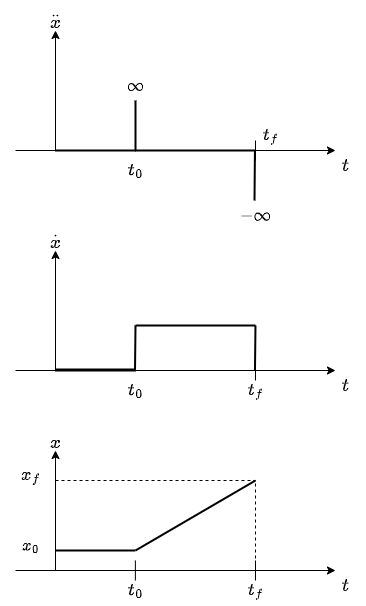
\includegraphics[keepaspectratio, scale=0.8]
      {images/png/inpulse.drawio.png}
 \caption{No continuity}
 \label{Fig:Step}
\end{figure}

ロボットの位置を変化させるには速度を出す必要がある.
初速度0m/sから目標速度までステップ状に変化させると時間に対する位置と加速度のグラフはFig\ref{Fig:Step}のようになる.
図を見ると加速度が無限大のインパルスを必要としていることがわかり,これは現実的ではない.
加速度が無限大のインパルスを必要としているのは,速度の変化がステップ状になっているからである.
すなわち,速度の変化量が無限になるからである.
ここからわかることは,速度は連続性が必要であるということである.
また,速度は位置の変化量であるため,位置も連続性が必要である.

このように速度に連続性のない制御は現実的ではないことがわかる.
逆に,加速度の連続性は必須ではないが加速度に1msぐらいの制御周期で連続性をもたせると,
なめらかな力制御を実現できる.

\newpage

%!TEX root = ../thesis.tex

\subsection{bang-bang制御}

\begin{figure}[H]
  \centering
 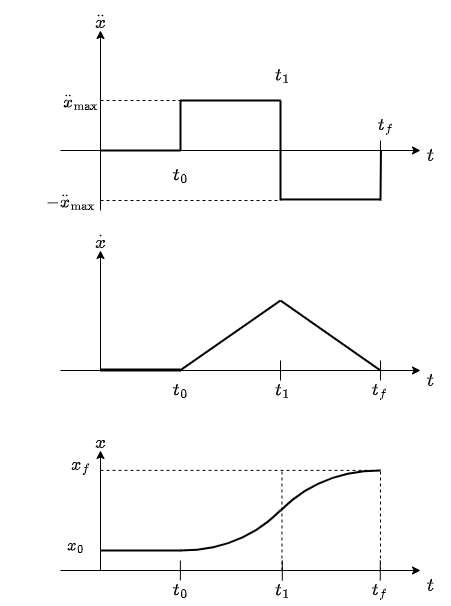
\includegraphics[keepaspectratio, scale=0.8]
      {images/png/bangbang.drawio.png}
 \caption{bang-bang control}
 \label{Fig:bangbang}
\end{figure}

速度に連続性をもたせた制御方式にbang-bang制御があり,最短時間軌道を達成できる.
最短時間軌道は,最速で目標地点に到達する際に有用な方法である.
bang-bang制御ではFig.\ref{Fig:bangbang}の加速度のグラフからわかるように,
最大加速と最小加速の2つの加速度をかけているため,最短時間で目標地点に到達することができる.
これは出発時にアクセルを全開にして,一気にブレーキをかけて,止まるというイメージである.

軌道生成及び制御を行うには初期値,目標値が必要である.今回は,位置xを変数とするため,初期値である初期位置を$x_0$,
目標値である目標位置を$x_f$,また,初速度$\dot{x}_0=0$,目標地点での速度$\dot{x}_f=0$とする.また,bang-bang制御は最大加速度$\ddot{a}_{max}$を必要とする.
このbang-bang制御を式で表すと以下のようになる.

\begin{equation} 
     \ddot{x} =
     \begin{cases}
          a & ( t_0 < t \leqq t_1 )\\
          -a & ( t_1 < t \leqq t_f )
     \end{cases}
\end{equation}

\begin{equation} 
     \dot{x} =
     \begin{cases}
          \dot{x}_0 + a(t -t_0) & ( t_0 < t \leqq t_1 )\\
          \dot{x}_1 + a(t - t_1) & ( t_1 < t \leqq t_f ) 
     \end{cases}
\end{equation}

\begin{equation}
     \text{ where $\dot{x}_1 = \dot{x}_0 + a(t_1 - t_0), \dot{x}_0 = 0$}\nonumber
\end{equation}

\begin{equation} 
     x =
     \begin{cases}
          x_0 + \frac{1}{2}a(t -t_0)^2 & ( t_0 < t \leqq t_1 )\\
          x_1 + \dot{x}_1(t-t_1) - \frac{1}{2}a(t - t_1)^2 & ( t_1 < t \leqq t_f )
     \end{cases}
\end{equation}

\begin{equation}
     \text{ where $x_1 = x_0 + \frac{1}{2}a\bigg\{\frac{(t_1 - t_0)}{2}\bigg\}^2$}\nonumber
\end{equation}

拘束条件を導出する.以上の3つの式を一般性を失わずに$t_0=0$とすると以下のようになる.

\begin{equation} 
     \ddot{x} =
     \begin{cases}
          a & ( t_0 < t \leqq t_1 )\\
          -a & ( t_1 < t \leqq t_f )
     \end{cases}
\end{equation}

\begin{equation}
     \text{ where $t_1 = \frac{t_f}{2}$}\nonumber
\end{equation}

\begin{equation} 
     \dot{x} =
     \begin{cases}
          at & ( t_0 < t \leqq t_1 )\\
          \dot{x}_1 - a(t - \frac{t_f}{2}) & ( t_1 < t \leqq t_f ) 
     \end{cases}
\end{equation}

\begin{equation} 
     \text{ where $\dot{x}_1 = a\frac{t_f}{2}$}\nonumber
\end{equation}

\begin{equation} 
     x =
     \begin{cases}
          x_0 + \frac{1}{2}at^2 & ( t_0 < t \leqq t_1 )\\
          x_1 + \dot{x}_1t - \frac{1}{2}at^2 & ( t_1 < t \leqq t_f )
     \end{cases}
\end{equation}

\begin{equation} 
     \text{ where $x_1 = x_0 + \frac{1}{2}a\Big(\frac{t_f}{2}\Big)^2$}\nonumber
\end{equation}

したがって,目標位置は
\begin{equation} 
     x_f = x_1 + \dot{x}_1t_f + a\frac{(t_f)^2}{2}
\end{equation}

となり,式(3.7)に$\dot{x}_1$,$x_1$を代入すると以下のようになる.
\begin{equation} 
     x_f = x_0 + \frac{1}{2}a\Big(\frac{t_f}{2}\Big)^2 + a\frac{t_f}{2}t_f + a\frac{(t_f)^2}{2}
\end{equation}

式(3.8)の$x_f$,$x_0$,は定数であり,変数は,目標地点への到達時間$t_f$と加速度$a$である.
最終到達時間$t_f$が決まると加速度aを求めることができ,すべての経路を決めることができる.
このときの加速度$a$は最大加速度$\ddot{x}_{max}$となる.

ここで,与える条件をまとめると以下のようになる.
\begin{description}
     \item[目標]\mbox{}\\
     $x_0, x_f$
     \item[拘束]\mbox{}\\
     $\dot{x_0}=0, \dot{x_f}=0, t_0=0, t_f$
\end{description}

\newpage
\begin{figure}[H]
     \centering
    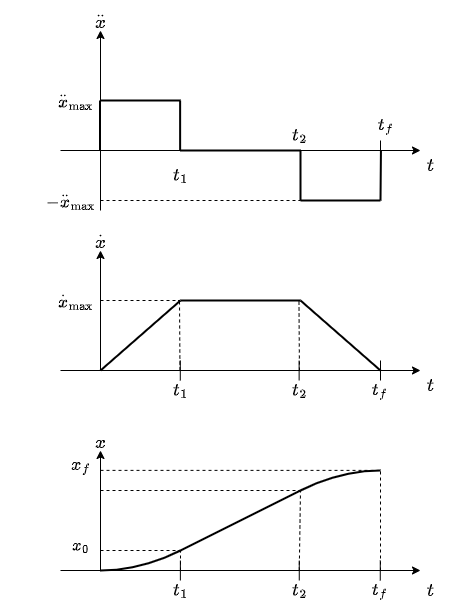
\includegraphics[keepaspectratio, scale=0.8]
         {images/png/bangbangV.drawio.png}
    \caption{bang-bang control with additional velocity constraints}
    \label{Fig:bangbangV}
\end{figure}
\newpage

bang-bang制御は加速度の変化に対応していないが,速度を変えることはできる.
拘束条件として,$\dot{x}_{max}$を追加すると,Fig.\ref{Fig:bangbangV}のようになる.
ここで$\dot{x}_{max}$は$\dot{x}_{max}=at_1$と求めることができる.
最短時間で最大速度を出すとき$\dot{x}_{max}=\ddot{x}_{max}t_1$となる.
目標地点到達時間$t_f$は$t_f=t_1+t_2$となり,$t_1$と$t_2$がわかれば,求めることができる.\\
$t_1$は$\dot{x}_{max}=\ddot{x}_{max}t_1$より\\
\begin{equation} 
     t_1=\frac{\dot{x}_{max}}{\ddot{x}_{max}}
\end{equation}
となる.\\
$t_0 < t \leqq t_1$のときの速度面積と$t_2 < t \leqq t_f$のときの速度面積は同じであるため,
$t_2$での距離は$t_0$から$t_2$までの速度が作り出す長方形の速度面積と同じになる.
したがって,$t_2$は
\begin{equation} 
     t_2=\frac{x_f-x_0}{\dot{x}_{max}}
\end{equation}
となる.\\
これにより,$\dot{x}_{max}$と$\ddot{x}_{max}$を求めることができる.

\newpage

%!TEX root = ../thesis.tex

\section{第3章のまとめ}

第3章ではbang-bang制御による軌道制御の解説を行った.速度と位置には連続性が必要であり,
拘束条件と目標を定める必要があった.bang-bang制御では最大加速度を求める必要があった.
また,速度が台形の場合の計算を行った.この場合は,拘束条件に最大速度を追加することで,
なだらかな速度変化を行えることを紹介した.

\newpage

%

%% Back Matter
\backmatter{}
%
%!TEX root = ../thesis.tex
%\bibliographystyle{plain}
\bibliographystyle{junsrt}
%\bibliography{report}
\nocite{*}
\bibliography{main_bibliography}
本レポートはインテリジェントロボットモーション第11回「軌道計画と軌道生成」の講義を元に制作した.
%

%

%

\end{document}
